\begin{figure*}[p]
  \centering
  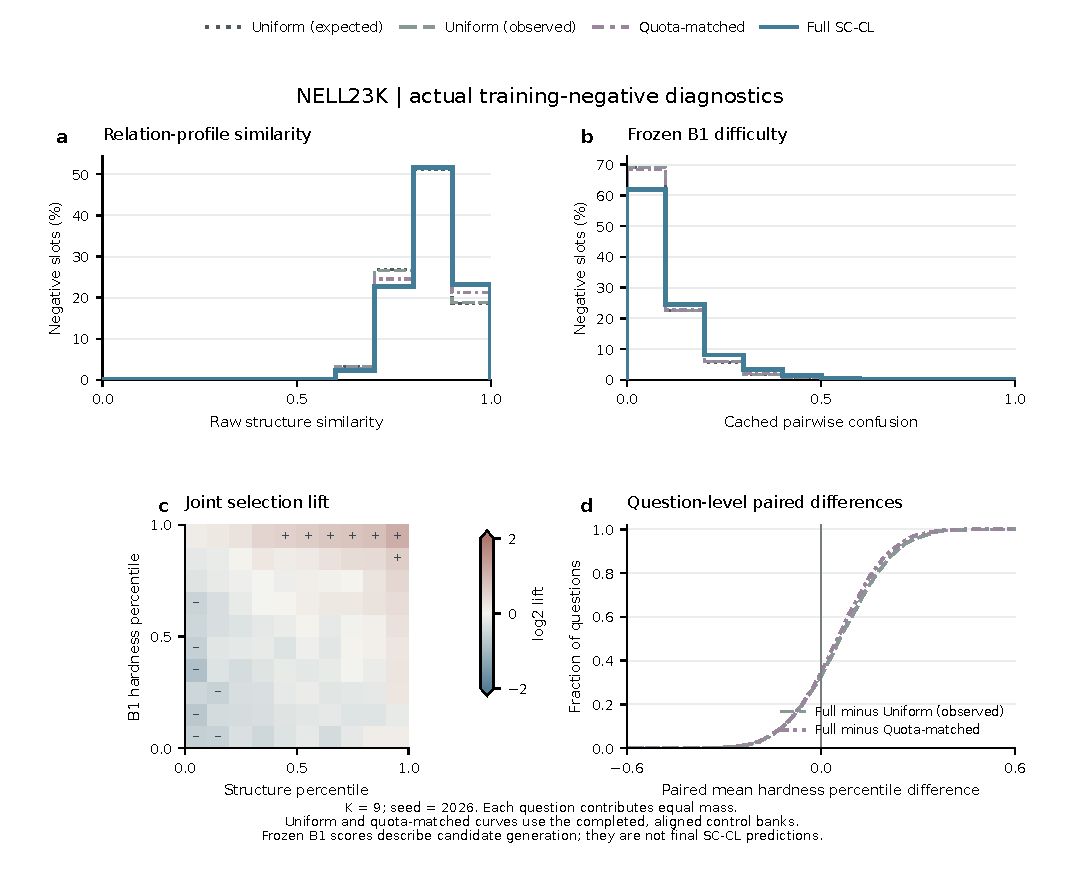
\includegraphics[width=\textwidth]{figures/sampling_diagnostics_seed2026/diagnostics_nell23k.pdf}
  \caption{NELL23K候选采样细图。a，关系画像结构相似度；b，缓存的冻结B1 pairwise confusion；c，相对逐题合法池解析Uniform的联合log2富集；d，Full与已训练均匀及频率配额匹配bank逐题平均困难度百分位的配对差异经验分布。每题等权，$K=9$，seed=2026。}
  \label{fig:sampling-diagnostics-nell}
\end{figure*}



\begin{figure*}[p]
  \centering
  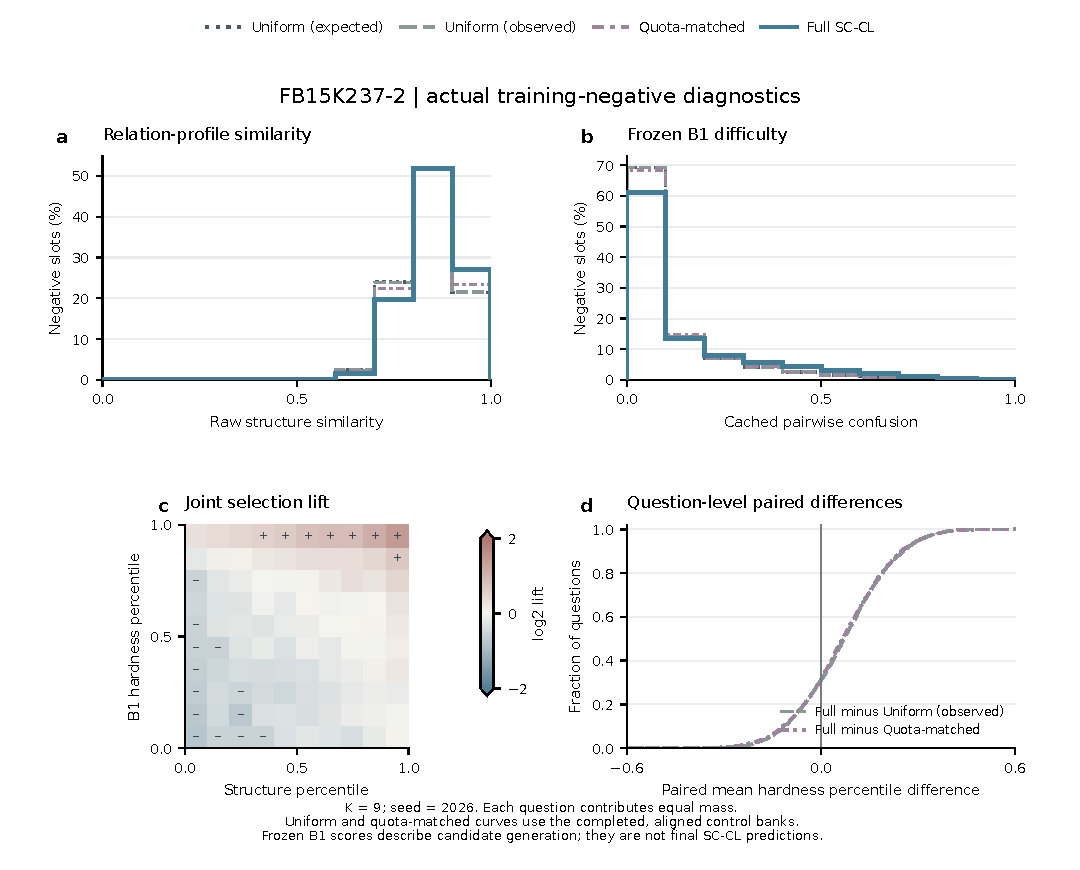
\includegraphics[width=\textwidth]{figures/sampling_diagnostics_seed2026/diagnostics_fb15k237_2.pdf}
  \caption{FB15K237-2候选采样细图。面板定义同图~\ref{fig:sampling-diagnostics-nell}；实际分布同时展示Full、均匀随机和配额匹配控制。所有候选来源均已完成且题目对齐。每题等权，$K=9$，seed=2026。}
  \label{fig:sampling-diagnostics-fb}
\end{figure*}

\begin{figure*}[p]
  \centering
  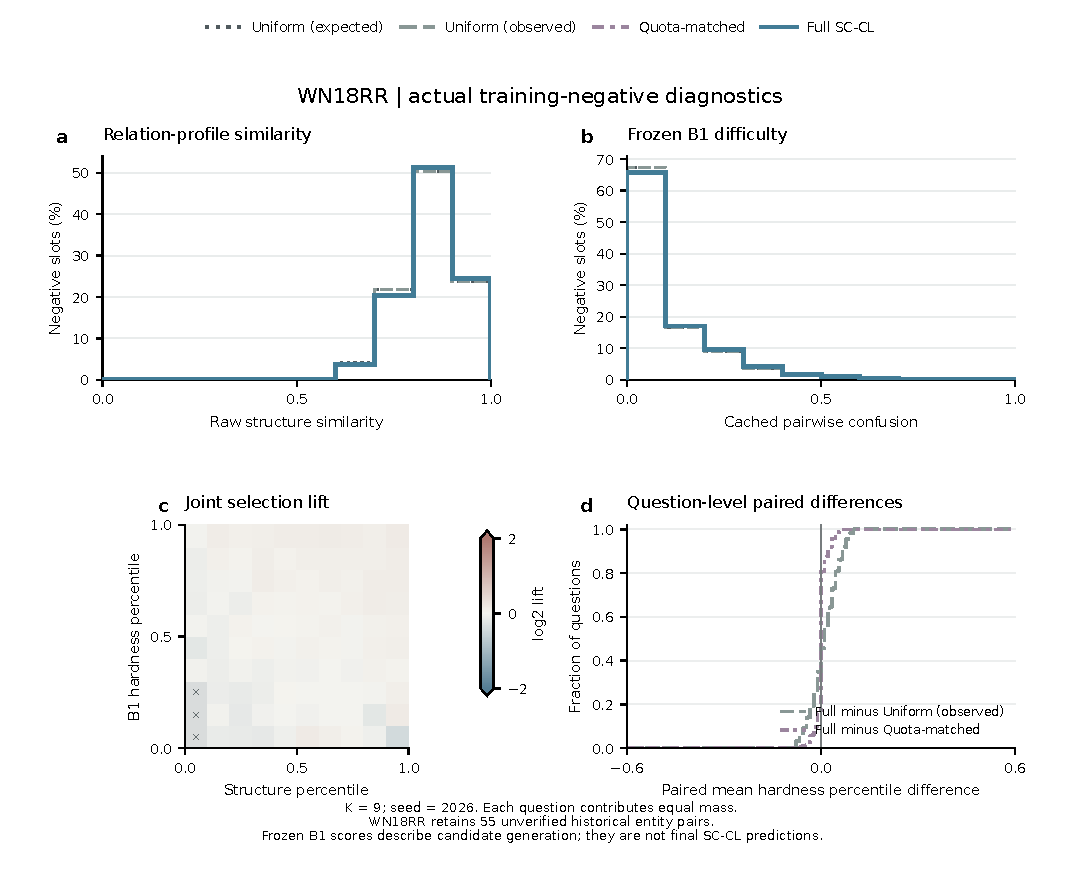
\includegraphics[width=\textwidth]{figures/sampling_diagnostics_seed2026/diagnostics_wn18rr.pdf}
  \caption{WN18RR候选采样细图。面板定义同图~\ref{fig:sampling-diagnostics-nell}；沿用历史候选池并保留55道实体对未核实问题。该数据集每题合法负关系数为9或10，$K=9$，因而题内rank百分位较离散；图为历史候选池条件下的单种子描述。}
  \label{fig:sampling-diagnostics-wn}
\end{figure*}
